% Created 2021-05-05 Wed 10:12
% Intended LaTeX compiler: pdflatex
\documentclass[11pt]{article}
\usepackage[utf8]{inputenc}
\usepackage[T1]{fontenc}
\usepackage{graphicx}
\usepackage{grffile}
\usepackage{longtable}
\usepackage{wrapfig}
\usepackage{rotating}
\usepackage[normalem]{ulem}
\usepackage{amsmath}
\usepackage{textcomp}
\usepackage{amssymb}
\usepackage{capt-of}
\usepackage{hyperref}
\usepackage[top=1in, bottom=1.25in, left=1.25in, right=1.25in]{geometry}
\usepackage{amsmath}
\usepackage{parskip}

\usepackage[main,include]{embedall}
\IfFileExists{./\jobname.org}{\embedfile[desc=The original file]{\jobname.org}}{}





\usepackage{fvextra}
\fvset{
  commandchars=\\\{\},
  highlightcolor=white!95!black!80!blue,
  breaklines=true,
  breaksymbol=\color{white!60!black}\tiny\ensuremath{\hookrightarrow},
}
\renewcommand\theFancyVerbLine{\footnotesize\color{black!40!white}\arabic{FancyVerbLine}}

\usepackage[many]{tcolorbox}
\DeclareTColorBox[]{Code}{}%
{enhanced,
  colback=white!97!black,
  colframe=white!94!black, boxrule=0.5pt,
  fontupper=\color{EFD}\footnotesize,
  arc=2.5pt, outer arc=2.5pt,
  boxsep=2pt, left=2pt, right=2pt, top=1pt, bottom=0.5pt,
  breakable}

\definecolor{EFD}{HTML}{383a42}
\newcommand{\EFD}[1]{\textcolor{EFD}{#1}} % default
\definecolor{EFk}{HTML}{e45649}
\newcommand{\EFk}[1]{\textcolor{EFk}{#1}} % font-lock-keyword-face
\definecolor{EFd}{HTML}{84888b}
\newcommand{\EFd}[1]{\textcolor{EFd}{\textit{#1}}} % font-lock-doc-face
\definecolor{EFt}{HTML}{986801}
\newcommand{\EFt}[1]{\textcolor{EFt}{#1}} % font-lock-type-face
\definecolor{EFs}{HTML}{50a14f}
\newcommand{\EFs}[1]{\textcolor{EFs}{#1}} % font-lock-string-face
\definecolor{EFw}{HTML}{986801}
\newcommand{\EFw}[1]{\textcolor{EFw}{#1}} % font-lock-warning-face
\definecolor{EFb}{HTML}{a626a4}
\newcommand{\EFb}[1]{\textcolor{EFb}{#1}} % font-lock-builtin-face
\definecolor{EFct}{HTML}{9ca0a4}
\newcommand{\EFct}[1]{\textcolor{EFct}{#1}} % font-lock-comment-face
\definecolor{EFc}{HTML}{b751b6}
\newcommand{\EFc}[1]{\textcolor{EFc}{#1}} % font-lock-constant-face
\definecolor{EFpp}{HTML}{4078f2}
\newcommand{\EFpp}[1]{\textcolor{EFpp}{\textbf{#1}}} % font-lock-preprocessor-face
\definecolor{EFnc}{HTML}{4078f2}
\newcommand{\EFnc}[1]{\textcolor{EFnc}{\textbf{#1}}} % font-lock-negation-char-face
\definecolor{EFv}{HTML}{6a1868}
\newcommand{\EFv}[1]{\textcolor{EFv}{#1}} % font-lock-variable-name-face
\definecolor{EFf}{HTML}{a626a4}
\newcommand{\EFf}[1]{\textcolor{EFf}{#1}} % font-lock-function-name-face
\definecolor{EFcd}{HTML}{9ca0a4}
\newcommand{\EFcd}[1]{\textcolor{EFcd}{#1}} % font-lock-comment-delimiter-face
\definecolor{EFrc}{HTML}{4078f2}
\newcommand{\EFrc}[1]{\textcolor{EFrc}{\textbf{#1}}} % font-lock-regexp-grouping-construct
\definecolor{EFrb}{HTML}{4078f2}
\newcommand{\EFrb}[1]{\textcolor{EFrb}{\textbf{#1}}} % font-lock-regexp-grouping-backslash
\definecolor{EFhn}{HTML}{da8548}
\newcommand{\EFhn}[1]{\textcolor{EFhn}{\textbf{#1}}} % highlight-numbers-number
\definecolor{EFhq}{HTML}{4078f2}
\newcommand{\EFhq}[1]{\textcolor{EFhq}{#1}} % highlight-quoted-quote
\definecolor{EFhs}{HTML}{986801}
\newcommand{\EFhs}[1]{\textcolor{EFhs}{#1}} % highlight-quoted-symbol
\definecolor{EFrdi}{HTML}{4078f2}
\newcommand{\EFrdi}[1]{\textcolor{EFrdi}{#1}} % rainbow-delimiters-depth-1-face
\definecolor{EFrdii}{HTML}{a626a4}
\newcommand{\EFrdii}[1]{\textcolor{EFrdii}{#1}} % rainbow-delimiters-depth-2-face
\definecolor{EFrdiii}{HTML}{50a14f}
\newcommand{\EFrdiii}[1]{\textcolor{EFrdiii}{#1}} % rainbow-delimiters-depth-3-face
\definecolor{EFrdiv}{HTML}{da8548}
\newcommand{\EFrdiv}[1]{\textcolor{EFrdiv}{#1}} % rainbow-delimiters-depth-4-face
\definecolor{EFrdv}{HTML}{b751b6}
\newcommand{\EFrdv}[1]{\textcolor{EFrdv}{#1}} % rainbow-delimiters-depth-5-face
\definecolor{EFrdvi}{HTML}{986801}
\newcommand{\EFrdvi}[1]{\textcolor{EFrdvi}{#1}} % rainbow-delimiters-depth-6-face
\definecolor{EFrdvii}{HTML}{4db5bd}
\newcommand{\EFrdvii}[1]{\textcolor{EFrdvii}{#1}} % rainbow-delimiters-depth-7-face
\definecolor{EFrdiix}{HTML}{80a880}
\newcommand{\EFrdiix}[1]{\textcolor{EFrdiix}{#1}} % rainbow-delimiters-depth-8-face
\definecolor{EFrdix}{HTML}{887070}
\newcommand{\EFrdix}[1]{\textcolor{EFrdix}{#1}} % rainbow-delimiters-depth-9-face
\author{Jake Moss - s46409665}
\date{\today}
\title{Project - Positional analysis of chess games}
\hypersetup{
 pdfauthor={Jake Moss - s46409665},
 pdftitle={Project - Positional analysis of chess games},
 pdfkeywords={},
 pdfsubject={},
 pdfcreator={Emacs 28.0.50 (Org mode 9.5)}, 
 pdflang={English}}
\begin{document}

\maketitle
\tableofcontents

\newpage

\section{Introduction}
\label{sec:org5ae5faa}
\subsection{Project aims}
\label{sec:orga506a2e}
The goal of this project was to provide a new and unique visualisation of chess games. To accomplish this two main plots where developed,

\begin{itemize}
\item Heat map of where pieces were captured
\item Histogram of when pieces were captured
\end{itemize}

The purpose of this project is to show the positional differences between different levels of play and in different time periods. This is something not often visualised within the chess community.
\subsection{Obtaining data}
\label{sec:orge5ab2bf}
\subsubsection{Sources}
\label{sec:org0c71eb1}
Chess games are found freely on the internet from many archives such as \href{https://www.pgnmentor.com/files.html}{PGN Mentor} and \href{https://www.ficsgames.org/download.html}{FICS Games Database}. From here I am able to download millions of games at mass. However, when considering large time periods most preserved games are of tournaments and high skill players, this data does not show the trends of average level games. To help mitigate this the \texttt{FISC} database was used to analyse a wide range of skill level games from a single year.
This tool was also build with the capability to analyse a single players games given their username from \href{https://lichess.org/}{Lichess} and \href{https://www.chess.com/}{Chess.com.} These games can be downloaded using their respective public API's.

To download games from \href{https://www.chess.com/}{Chess.com} the bash command below can be used.
\begin{Code}
\begin{Verbatim}[]
\color[HTML]{383a42}\EFk{for} g\EFk{ in} \$\textcolor[HTML]{4078f2}{(}\textcolor[HTML]{986801}{curl} -Ls https://api.chess.com/pub/player/\$\EFv{PLAYERNAME}/games/archives | jq -rc \EFs{".archives[]"}\textcolor[HTML]{4078f2}{)} ; \EFk{do} \textcolor[HTML]{986801}{curl} -Ls \EFs{"}\textcolor[HTML]{b751b6}{\$}\textcolor[HTML]{6a1868}{g}\EFs{"} | jq -rc \EFs{".games[].pgn"} ; \EFk{done} >> games.pgn
\end{Verbatim}
\end{Code}

Lichess easily allows for downloading of an entire players archive at once with a simple \texttt{curl}.
\begin{Code}
\begin{Verbatim}[]
\color[HTML]{383a42}\textcolor[HTML]{986801}{curl} https://lichess.org/games/export/\$\EFv{PLAYERNAME} > games.pgn
\end{Verbatim}
\end{Code}

\texttt{DaenaliaEvandruile} has given their permission for their games to be featured with this report to demonstrate this functionality.
\subsubsection{PGN Format}
\label{sec:org63aa24e}
The most common format used to store chess games is \href{https://en.wikipedia.org/wiki/Portable\_Game\_Notation}{Portable Game Notation}. It is a human-readable plain text notation which stores individual moves rather than the board states. While this is considerably more efficient for both storage and transcribing it makes extracting data that isn't explicitly given difficult and costly.

The \href{http://www.saremba.de/chessgml/standards/pgn/pgn-complete.htm}{PGN standard} defines a required \href{http://www.saremba.de/chessgml/standards/pgn/pgn-complete.htm\#c8.1.1}{seven tag roster} and allows for optional tags such as \texttt{WhiteElo} and \texttt{BlackElo}. Each move is stored in \href{https://en.wikipedia.org/wiki/Algebraic\_notation\_(chess)}{Standard Algebraic Notation}, which describes the change in board state such as captures, checks, and promotions.

SAN comes in a varsity of formats short, long, or minimal. Each variant encodes moves with different levels of detail. Unfortunately no single variant is used in all PGN databases, although it is rare for the format to change from within a database.

A standard game might look something like this
\begin{verbatim}
[Event "WCh 2018"]
[Site "London ENG"]
[Date "2018.11.09"]
[White "Caruana, Fabiano"]
[Black "Carlsen, Magnus"]
[Result "1/2-1/2"]
[WhiteTitle "GM"]
[BlackTitle "GM"]
[WhiteElo "2832"]
[BlackElo "2835"]
[WhiteFideId "2020009"]
[BlackFideId "1503014"]
[EventDate "2018.11.09"]

1. e4 c5 2. Nf3 Nc6 3. Bb5 g6 ... 115. Ra8 1/2-1/2
\end{verbatim}
Game tags must be in \texttt{[]}. Often there are more than the standard requires. These tags are referred to as the headers. The moves themselves are listed in SAN with the result at the end.
\section{Data Processing}
\label{sec:org09de8f2}
\subsection{Tools used}
\label{sec:orgf57b4a6}
This project made use of the below tools,
\begin{itemize}
\item \href{https://github.com/niklasf/python-chess}{python-chess}
Used to handle the complex move validation and PGN parsing required to step though games.
\item \href{https://matplotlib.org/}{matplotlib}
Standard plotting library.
\item \href{https://seaborn.pydata.org/}{seaborn}
A high level plotting library built on \texttt{matplotlib}.
\item \href{https://numpy.org/}{numpy}
Standard scientific computing library. Within this project it is used for its \texttt{pandas} optimisations, and reshape function.
\item \href{https://pandas.pydata.org/}{pandas}
Data frames provide an efficient way to store and conditionally select games based on metadata.
\item \href{https://github.com/python/cpython}{cPython Profiler}
Function call profiler.
\item \href{https://jiffyclub.github.io/snakeviz/}{snakeViz}
In browser \texttt{cPython profiler} visualiser.
\end{itemize}

\subsection{Meta Data Extraction}
\label{sec:org9f3c667}
To extract the metadata from a game the PGN file is read using standard python methods and the game object is initialised using the \texttt{aggergate} function from the \texttt{aggergation.py} module. From the game object the headers are extracted into a dictionary and a data frame is created consisting of the headers as column titles and rows as individual games.

\begin{center}
\begin{tabular}{lllllllll}
 & SAN string & Black & White & Result & BlackElo & WhiteElo & Date & \ldots{}\\
\hline
1 & \texttt{string} & \texttt{string} & \texttt{string} & \texttt{string} & \texttt{int} & \texttt{int} & \texttt{DateTime} & \ldots{}\\
\ldots{} &  &  &  &  &  &  &  & \\
\end{tabular}
\end{center}

\subsection{Extracting Implicit Data}
\label{sec:orgbf80c9c}
To extract the ``implicit data'', such as piece captures, each game must be played out in its entirety with each move analysed as the format games are encoded and does not explicitly provided this information.

This data is then appended to the metadata data frame in another column. This allows for each conditioning of the data frame.
\section{Data Analysis}
\label{sec:org8db77bd}
\subsection{Local and Global Normalisation}
\label{sec:org66280c0}
Within the heat map grid plots, each map shares the colour bar on the right. To accomplish this each square with each map is normalised to the sum of the local grid so the map represents proportion instead of frequency. From this we now know the maximum value is \texttt{1} and the colour bar can be calibrated to \texttt{[0,1]}. However, as the proportion of lost pieces rarely gets close to \texttt{0.5} let alone \texttt{1}, the colours become hard to differentiate.

To remedy this I set the maximum of all local maximums to the max of the colour bar. This made it so that each plot is proportional to itself and the colouring is consistent between plots.

\begin{center}
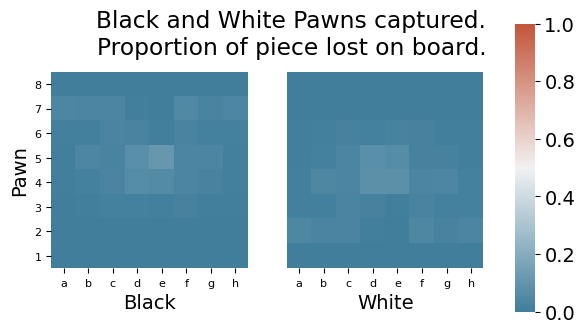
\includegraphics[width=0.4\textwidth]{Images/DaenaliaEvandruile_HEATMAP_Pawn_WHITE_EXAMPLE_1_WITH_WRONG_COLOUR.png}
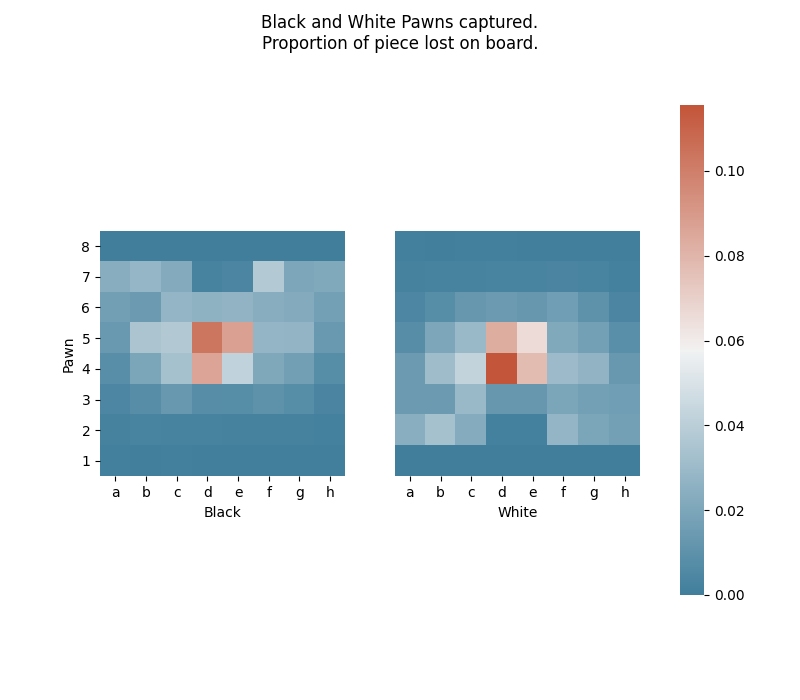
\includegraphics[width=0.4\textwidth]{Images/_HEATMAP_Pawn_FISC.png}
\end{center}
A similar strategy was employed to ensure the histograms and kernel density plots shared the same axis.

\newpage
\subsection{Piece comparability}
\label{sec:orga4be1a2}
As there are \(8\) pawns, but only \(1\) queen it is not fair to directly compare proportion statistics. This was not accounted for on purpose as doing so could muddy the information and may introduce over correction. Instead it is assumed that the viewer understands the context of the pieces.
\subsection{Colour schemes}
\label{sec:org8abaedb}
Although all plots presented here feature the same colour scheme for consistency, they are interchangeable with ease through the use of \texttt{matplotlib colour palettes}. Some example can be found \href{https://seaborn.pydata.org/tutorial/color\_palettes.html}{here}. This facilitates for adjustment due to the display medium and user accommodations. A grey scale can be used for printing, or appropriate pallets for colour blindness.

\begin{figure}[htbp]
\centering
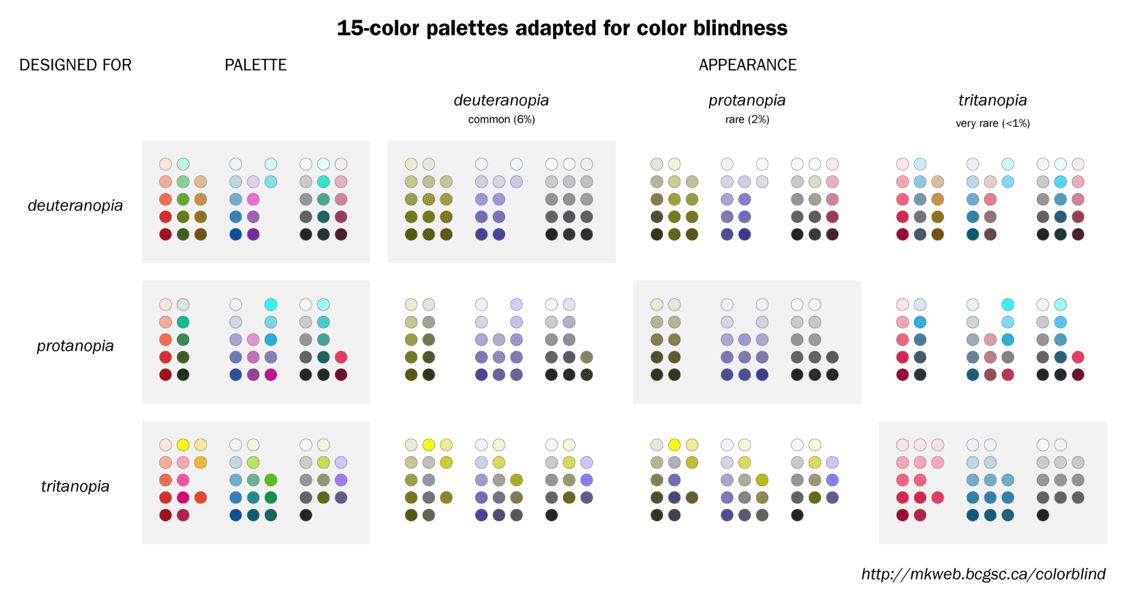
\includegraphics[width=\textwidth]{Images/color-blind-friendly-palette-9.png}
\caption{\href{https://mkweb.bcgsc.ca/colorblind/}{Image source}}
\end{figure}

All plot commands support supplying a custom \texttt{cmap} as an optional argument.
\section{Results}
\label{sec:orgba64c7d}
\begin{wrapfigure}[4]{r}{0.4\textwidth}
\centering
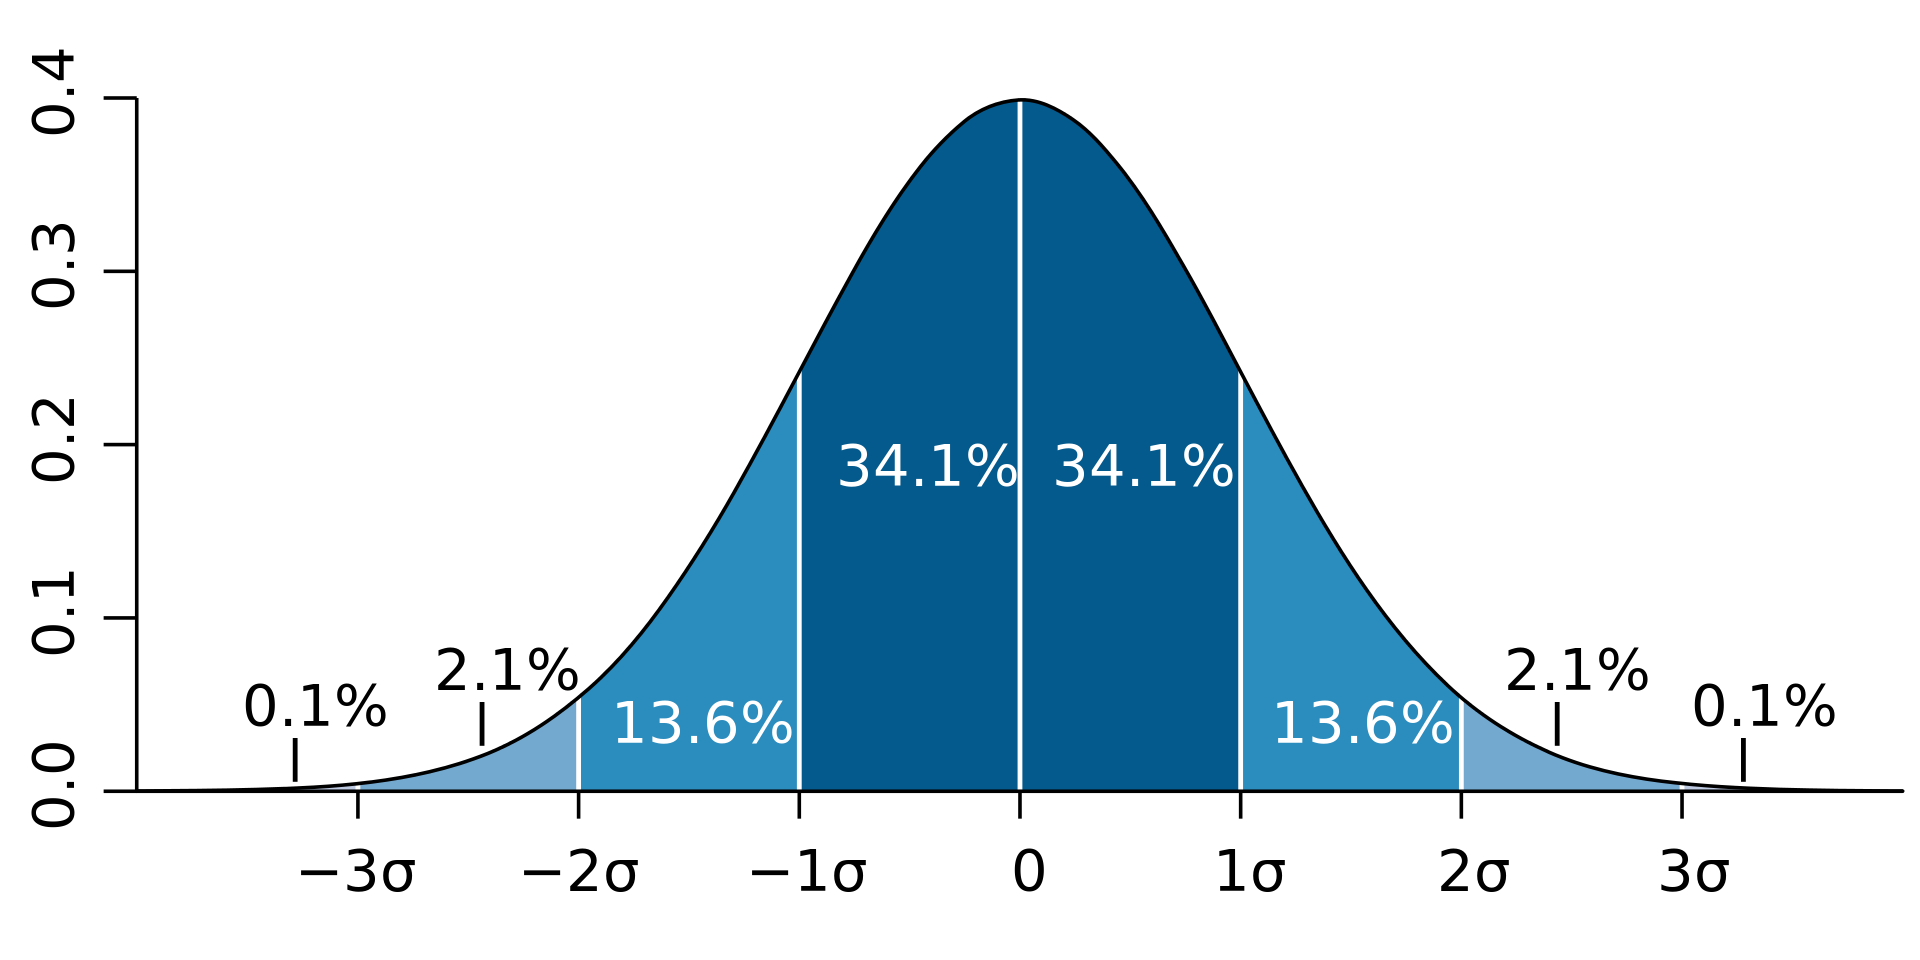
\includegraphics[width=0.3\textwidth]{Images/1920px-Standard_deviation_diagram.png}
\end{wrapfigure}
The skill level of players was assumed to be normally distributed. All ELO grid plots have their \texttt{x-axis} binned by percentiles from the normal distribution. Sigma or \(\sigma\) here denotes one standard deviation \cite{NormalDist}.
Date grid plots are binned by quartiles.

\subsection{Plot analysis}
\label{sec:orga6c680a}
\subsubsection{ELO grid plots}
\label{sec:org235ccac}
This first visualisation shows positions where pieces were lost by a particular colour plotted against ELO ranking of the player. Each combination of ELO and piece is represented by an \texttt{8x8} heat map of the board from Whites perspective. The decision to make all plots from Whites POV was made in an attempt to improve comparability and consistency between plots.
\begin{wrapfigure}[10]{l}{0.6\textwidth}
\centering
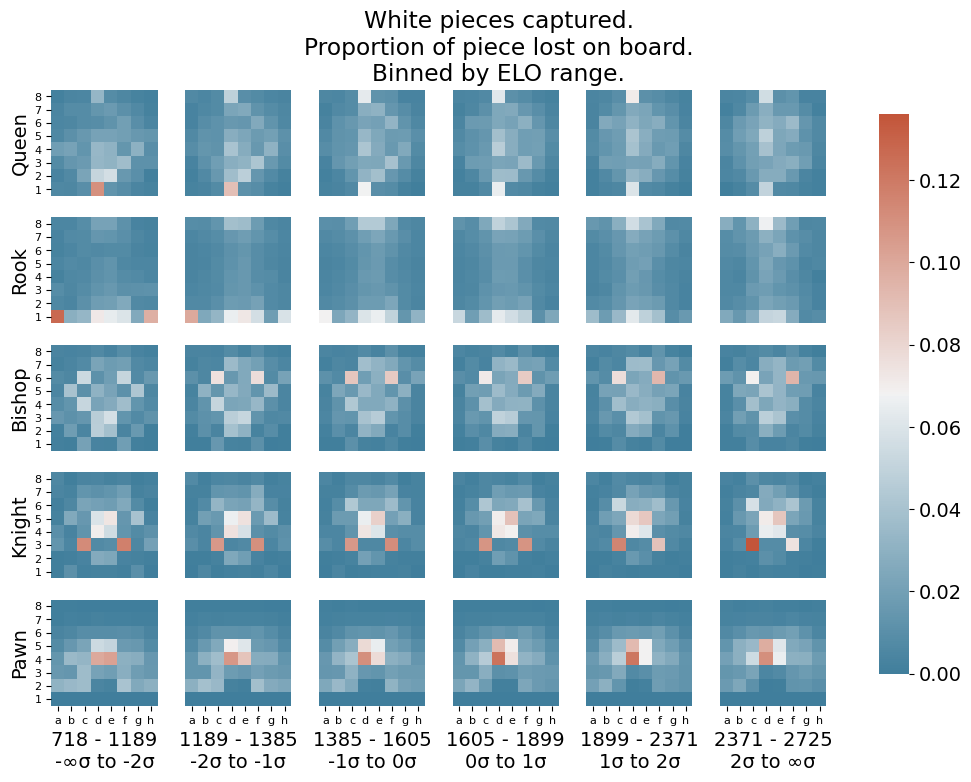
\includegraphics[width=0.5\textwidth]{Images/_HEATMAP_Queen_Rook_Bishop_Knight_Pawn_WHITE_ELO_FISC.png}
\caption{All captured White pieces binned by ELO}
\end{wrapfigure}

The unique pattern for each piece shows the most common lines played by White.

Queens typically move through the \texttt{C,D,E} pawns which are the easiest lines out of the starting position.
\begin{center}
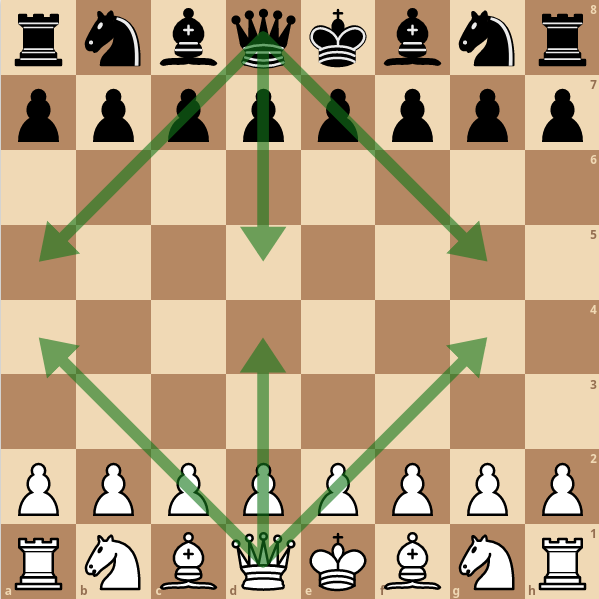
\includegraphics[width=100pt]{Images/Queen lines.png}
\end{center}

As ELO increases all pieces trend towards the centre as it is a highly advantageous position. The \texttt{A1} and \texttt{H1} Rooks (\texttt{A8} and \texttt{H8} for Black) loses almost disappear in higher ELO's, this is likely due to higher usage, and the utilisation of castling. The highest ELO players show a significant increase in spread of loses indicating that the Rooks are more active through a wider range of centre files.
The decrease in loses on positions that are common from castling does not indicate a decrease in castling as the heat maps only show losses, as higher ELO players are more likely to play better positions, they are less likely to castle into a position where their Rook will be lost.

A similar spread increase can be seen in the Queens. Higher ELO players tend to lose their Queens in a much more even manner. This may be a symptom of sacrificing which is common in high level play.

Bishops, Knights, and Pawns do not display a pattern change between ELOs suggesting most players know common and effective positioning. These position are common knowledge and often taught. Although there is negligible change in the patterns, the frequency at which they are lost becomes more concentrated. This may indicate that higher ELO player are more likely to keep these pieces near positions where they are strongest.

A similar plot as \texttt{Figure 1} is attached in the \hyperref[sec:orgac6d72f]{Appendix} which instead shows Black pieces. There is no note worthy pattern difference between the Black and White plot. All treads are present but with \(180^{\circ}\) rotation.

\begin{figure}[htbp]
\centering
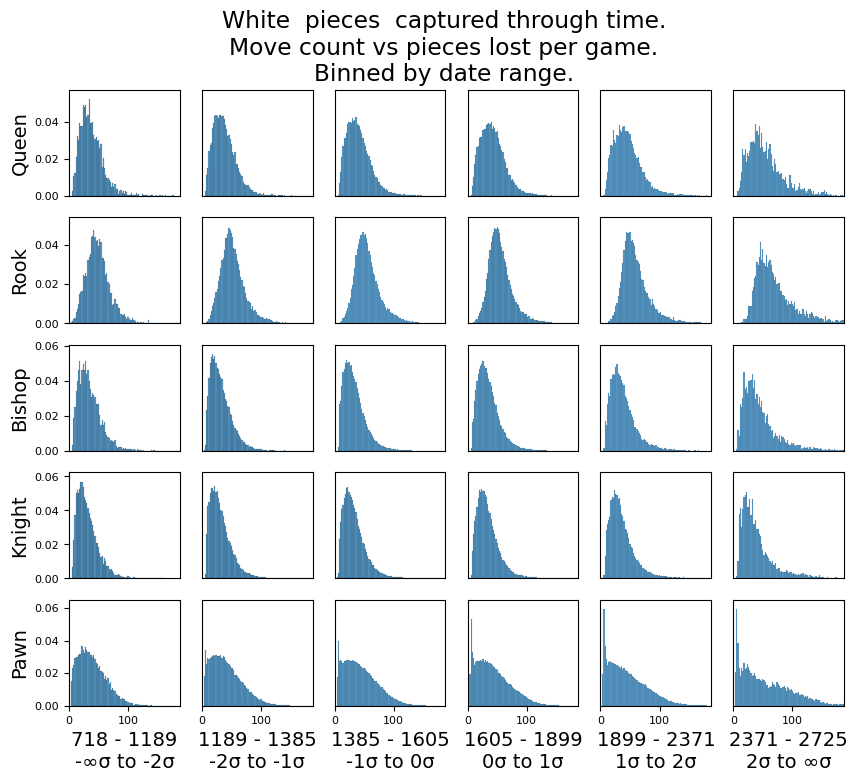
\includegraphics[width=0.7\textwidth]{Images/_HIST_Queen_Rook_Bishop_Knight_Pawn_WHITE_ELO_FISC.png}
\caption{When White pieces where captured binned by ELO}
\end{figure}

Here the number of captured pieces is divided by the number of games in the respective bin. This is to account for the different game counts due to the binning of players based on the assumption ELO is normally distributed.

Although there are a lower number of games in the more extreme percentiles (\texttt{col 1} and \texttt{col 6}) some conclusions can still be drawn.
A common trend among must all pieces is the gradual spreading effect of pieces lost per game. This is probably due to higher skill players playing longer games.
There is often a large spike in Pawn losses around move numbers \texttt{1-6} demonstrating the trading that is common at the beginning of games while competing for control of the centre of the board. This is corroborated by \texttt{Figure 1} where the Queen side Pawn is most commonly lost.

Further plots are included in the appendix.
\subsubsection{Date grid plots}
\label{sec:orgd9d82d5}
A different database was used for date binning as the \texttt{FISC} database only had games from \texttt{2000}, instead a database comprising of \texttt{Tournaments}, \texttt{Candidates} \texttt{Interzonals}, and \texttt{World Championships} games were used. (These games were acquired from \href{https://www.pgnmentor.com/files.html\#events}{PGN mentor}.)

\begin{center}
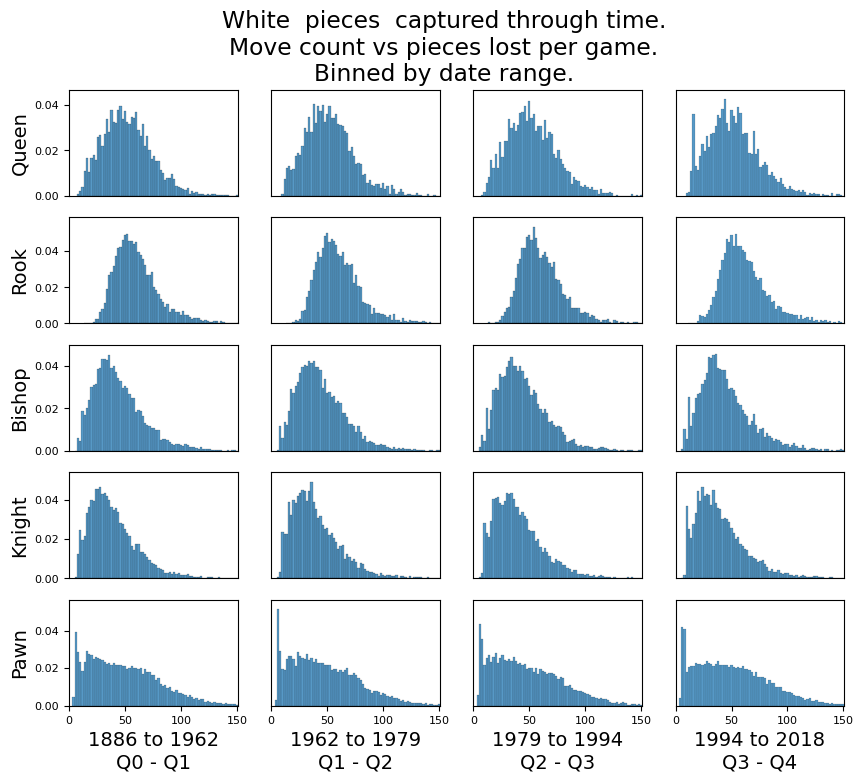
\includegraphics[width=0.7\textwidth]{Images/_HIST_Queen_Rook_Bishop_Knight_Pawn_WHITE_DATE_TOURNEMENTS.png}
\end{center}

Unfortunately binning by date reveals no interesting patterns or trends. However, it does show that chess has not changed significantly over the centuries.

Further plots are included in the appendix.

\subsubsection{Individual piece plots}
\label{sec:org6ba02a5}
Left hand side plots are from the \texttt{FISC} database. Right hand side from the \texttt{Tournements} database.
\begin{center}
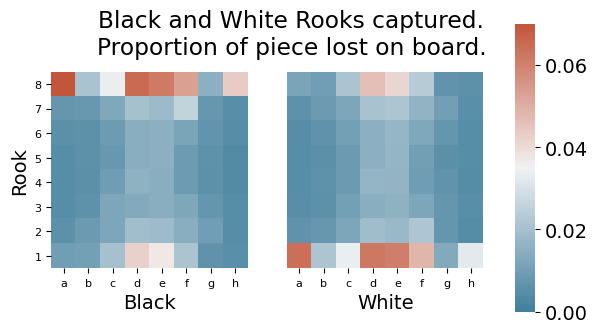
\includegraphics[width=0.45\textwidth]{Images/_HEATMAP_Rook_FISC.png}
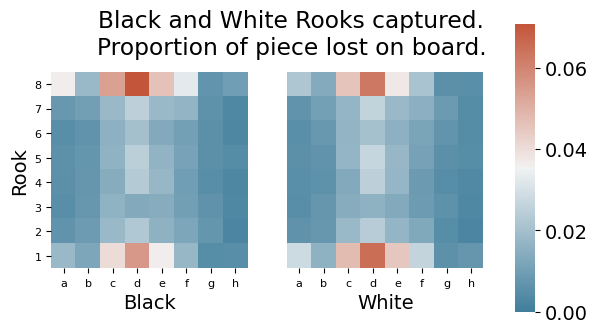
\includegraphics[width=0.45\textwidth]{Images/_HEATMAP_Rook_TOURNEMENTS.png}
\end{center}

\begin{center}
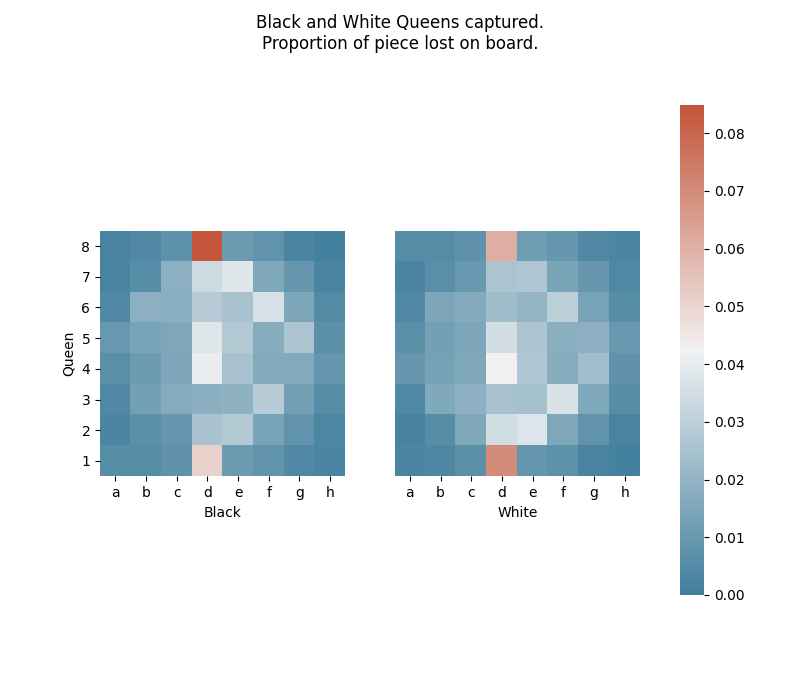
\includegraphics[width=0.45\textwidth]{Images/_HEATMAP_Queen_FISC.png}
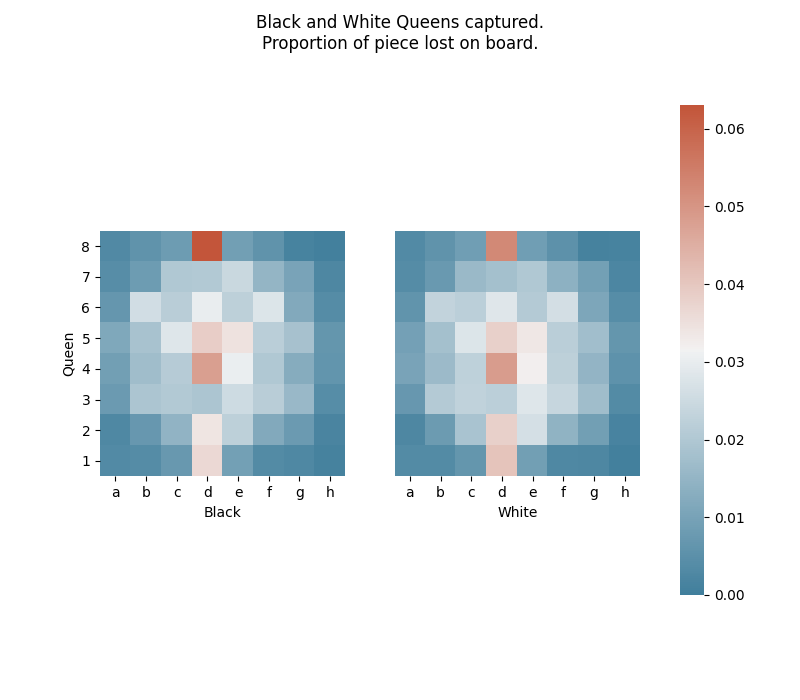
\includegraphics[width=0.45\textwidth]{Images/_HEATMAP_Queen_TOURNEMENTS.png}
\end{center}

As the \texttt{FISC} database contains varying skill level players, it is fair to assume the most prominent trends are those of average skill players, similar to the left side of \texttt{Figure 1}. The \texttt{Tournement} plots exhibit patterns similar to those of higher ELOs in \texttt{Figure 1} as expected.

High level players lose their Queens in the same positions regardless of colour. This could be a consequence of the \href{https://en.wikipedia.org/wiki/First-move\_advantage\_in\_chess}{first move advantage}.
\subsubsection{Individual player plots}
\label{sec:org9debea8}
All previously shown plots are also capable of focusing on a single player. Here we have positions where \texttt{DaenaliaEvandruile}'s Rooks were lost, and a histogram of when their Pawns were lost. This allows the user to compare their specific play patterns to common trends.

\begin{center}
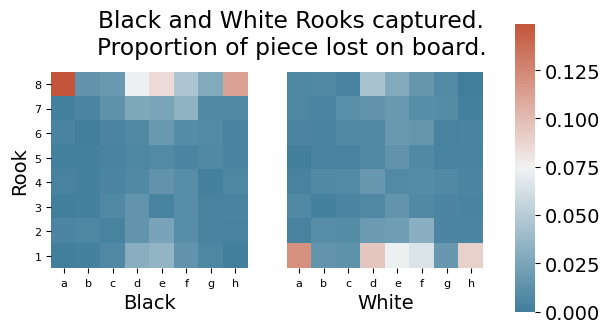
\includegraphics[width=0.45\textwidth]{Images/DaenaliaEvandruile_HEATMAP_Rook.png}
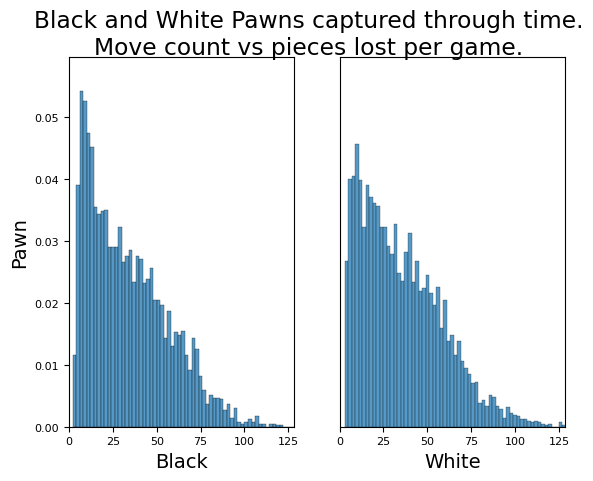
\includegraphics[width=0.45\textwidth]{Images/DaenaliaEvandruile_HIST_Pawn.png}
\end{center}
\subsection{Conclusion}
\label{sec:orge86b719}
Overall this project has successfully visualised an uncommon statistic of chess which may provide insight into future trends or an individual players style.

While the \texttt{Date} binning did not reveal and trends and patterns initially hoped for it was successful in showing the common positions do not often change over centuries.

All code and resources used are open source and is available at \href{https://github.com/Jake-Moss/chess-analysis}{this repository.}
\subsubsection{Areas for improvement}
\label{sec:org455a30f}
\begin{itemize}
\item Performance and memory requirements prevented me from analysing the databases I hoped to. A custom PGN parse and a rewrite of the main processing module in a language with more control over memory and data structures such as Rust or Haskell might provide the improvements required.
\item More positional statistics such as, positions that give and receive checks and checkmates may be interesting to visualise. This is possible with the current implementation requiring only a few more functions due to the features of the \texttt{python-chess} library and composability of my program.
\end{itemize}
\subsubsection{Flaws and disappointments}
\label{sec:orgc14c26e}
\begin{itemize}
\item I found myself struggling to manage the code base due to significant my lack of planning and documentation. In an effort to mitigate this I conducted 3 rewrites, each adding or changing significant portions of code.
\begin{itemize}
\item The first implementation had no storage of meta data or any way to filter game. Games where stored in a list and every plot had to play every game every time some new piece of information of required.
\item Second implementation used \texttt{5-6} lists to store meta data and filter the games. However managing \(5\) or \(6\) independent lists based on index alone wasn't easy to work with or scalable.
\item Final refactor added data frames and smarter processing. However, this had significant performance costs due to the magnitude of information that had to persist the life time of program and required a large portion of code to be rewritten to be compatible with data frames.
\end{itemize}
\end{itemize}

\section{Reflection}
\label{sec:orgaa8eb12}
As the program was designed with modularity and composability in mind it is highly general, and able to process any game database format and group based on any meta data field with a few changes. Binning based on location or opening would only require a few lines to group the games and the rest can remain unchanged.

No pre-processing is required by the user, all plots are non-specific to a single database. Everything is self contained making it easy to work with. Analysing another database requires a single filename change.
While writing this program my goal was not to visualise a single data set but rather to write a tool that allowed visualisation to be made with ease. This added a lot of complexity and time requirements, however, I believe this was for the best as it forced me to focus on the process itself rather than manipulate a single database.

While this program can create interesting and new visualisations, as far as I can see there is little strategical use for these plots. Single player can be created to show changes in piece positioning at current and previous rankings. However, plain positioning is unlikely to get you far in a game, complex theory and strategies play a much more important role.

An alternative project maybe to visualise evaluations of moves over time using an chess engine and table base. This could show differences in move accuracy and how the accuracy of different ELO's have changed.

Due to the complexity, design approach, and extent of this project, I believe it is deserving of a \(7\).
\newpage
\bibliographystyle{plain}
\bibliography{ref}
\newpage
\section{Appendix}
\label{sec:orgac6d72f}
\href{https://github.com/Jake-Moss/chess-analysis/tree/master/Images}{This repository} is the best place to view these images, under the \texttt{Images/} folder as well as the source code for this project. \texttt{main.py} contains all plots shown here.
\subsection{ELO Grids (FISC)}
\label{sec:orge7d6145}
\begin{center}
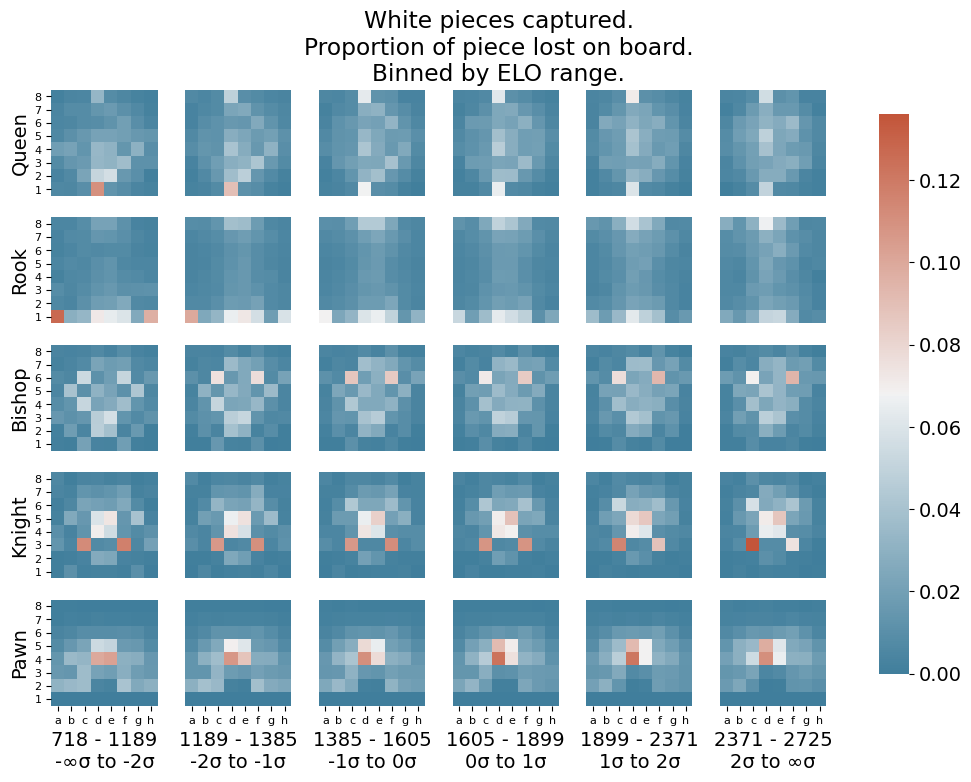
\includegraphics[width=\textwidth]{Images/_HEATMAP_Queen_Rook_Bishop_Knight_Pawn_WHITE_ELO_FISC.png}
\end{center}

\begin{center}
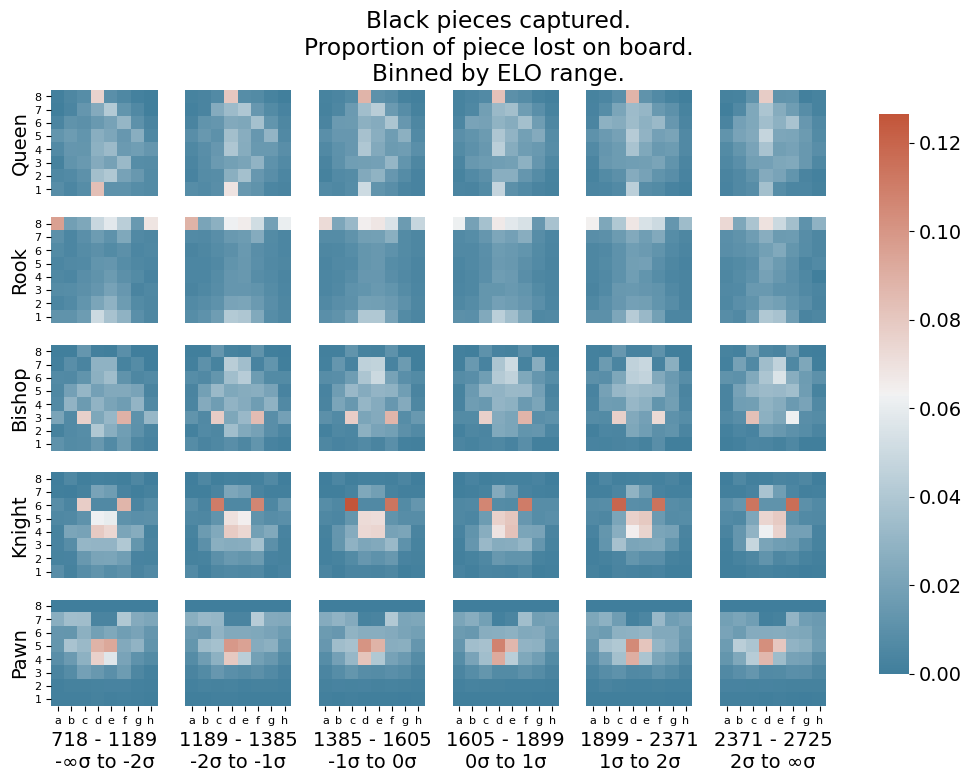
\includegraphics[width=\textwidth]{Images/_HEATMAP_Queen_Rook_Bishop_Knight_Pawn_BLACK_ELO_FISC.png}
\end{center}


\begin{center}
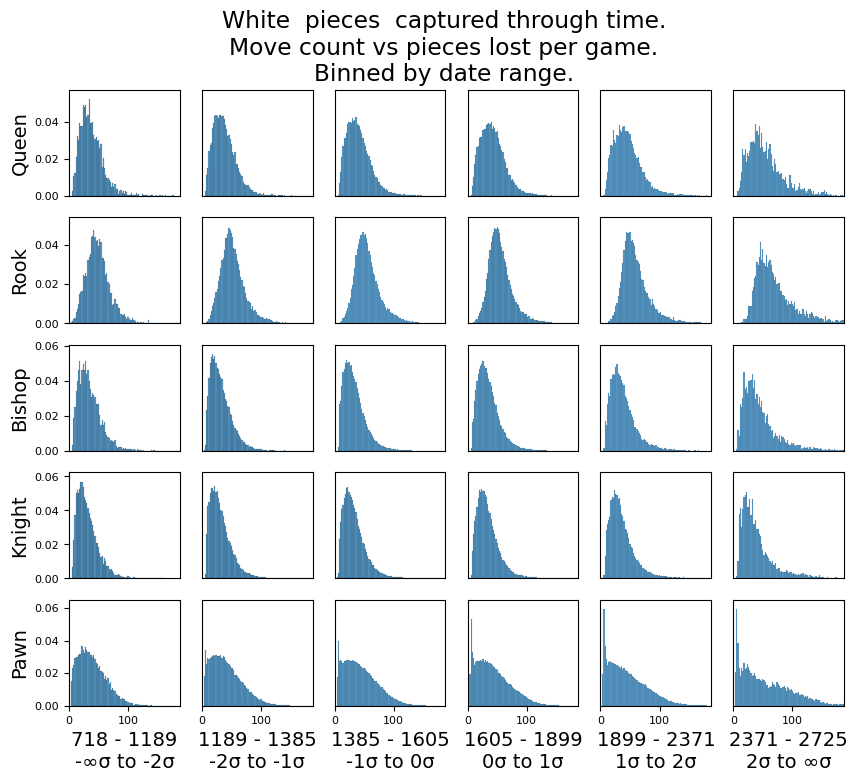
\includegraphics[width=\textwidth]{Images/_HIST_Queen_Rook_Bishop_Knight_Pawn_WHITE_ELO_FISC.png}
\end{center}

\begin{center}
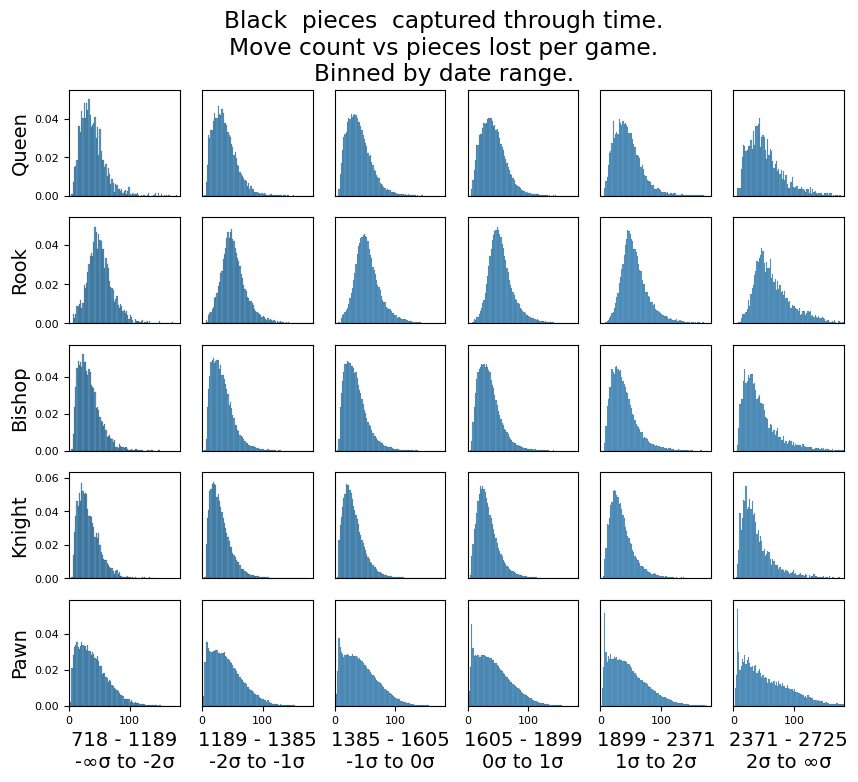
\includegraphics[width=\textwidth]{Images/_HIST_Queen_Rook_Bishop_Knight_Pawn_BLACK_ELO_FISC.png}
\end{center}

\subsection{Date Grids (Tournament)}
\label{sec:org23de98f}
\begin{center}
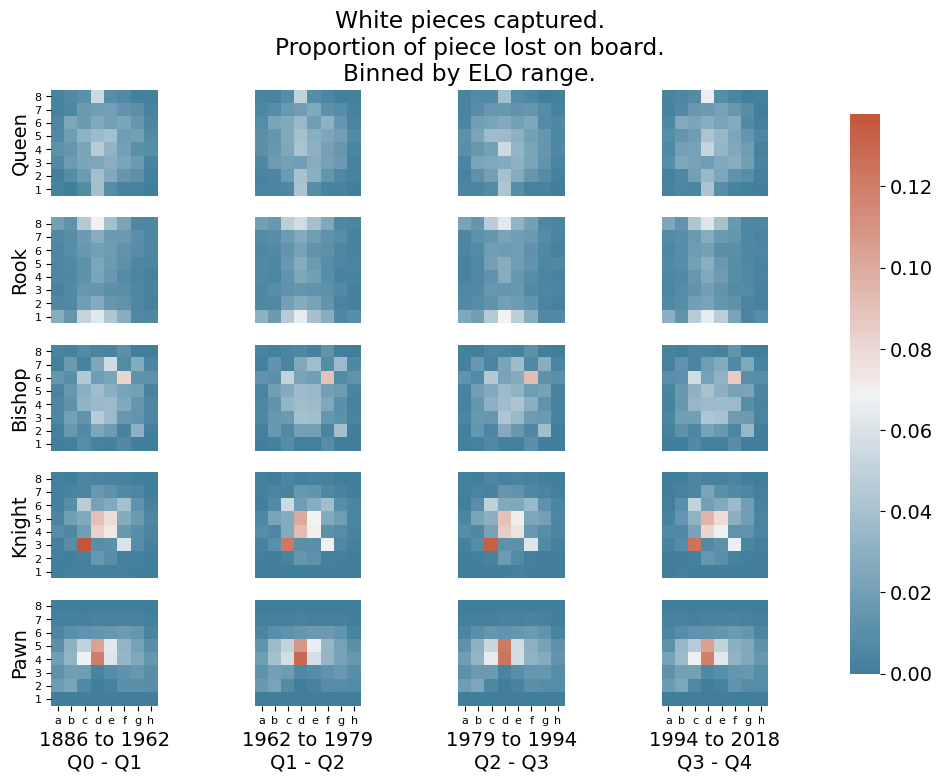
\includegraphics[width=\textwidth]{Images/_HEATMAP_Queen_Rook_Bishop_Knight_Pawn_WHITE_DATE_TOURNEMENTS.png}
\end{center}

\begin{center}
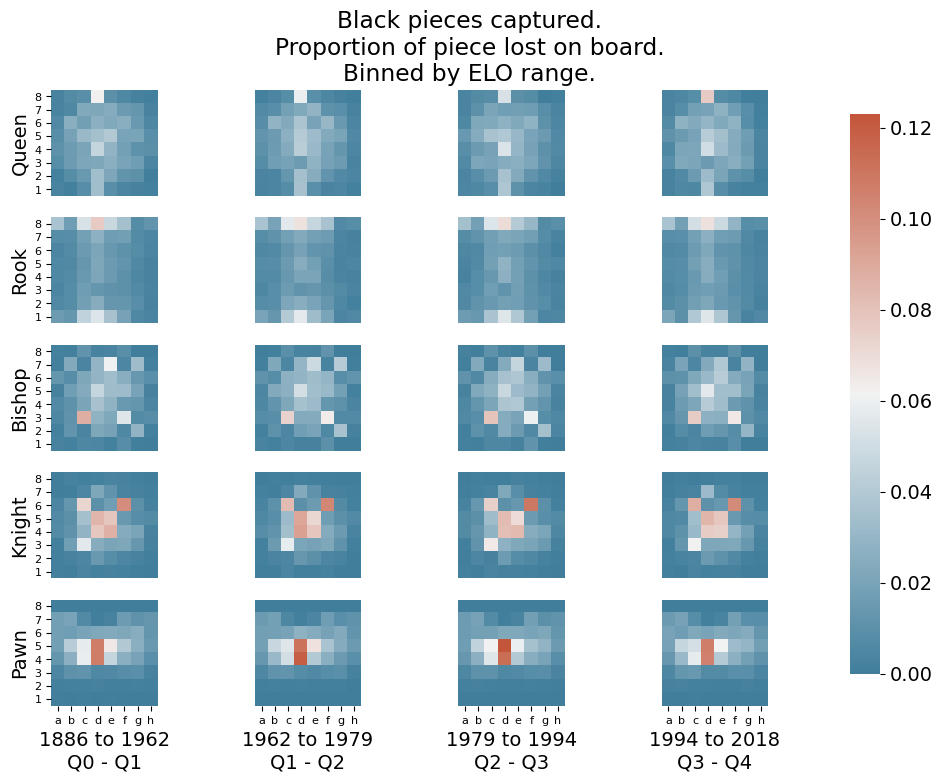
\includegraphics[width=\textwidth]{Images/_HEATMAP_Queen_Rook_Bishop_Knight_Pawn_BLACK_DATE_TOURNEMENTS.png}
\end{center}


\begin{center}
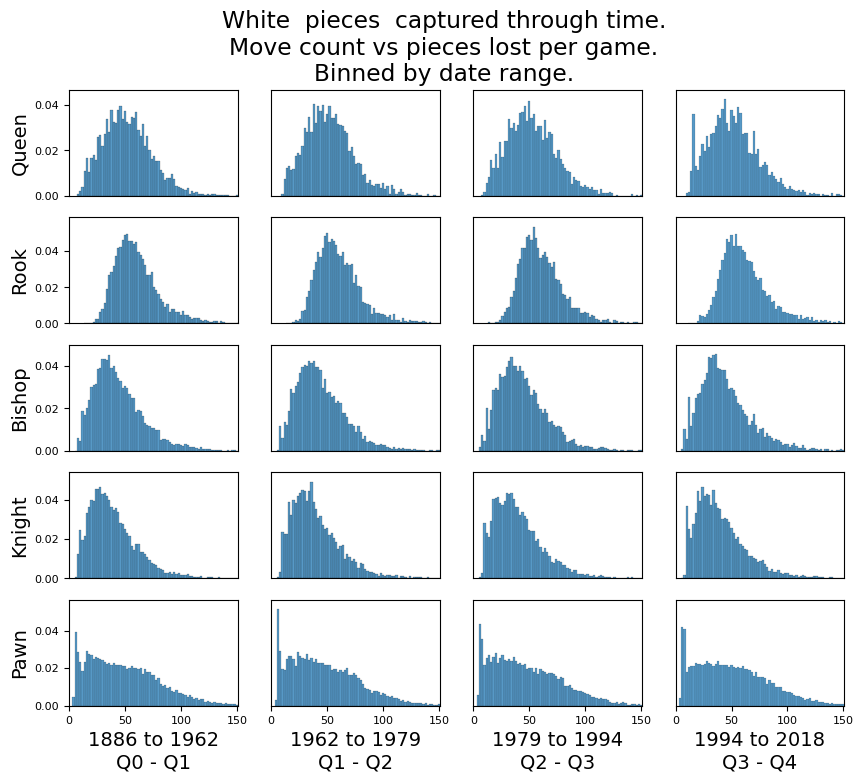
\includegraphics[width=\textwidth]{Images/_HIST_Queen_Rook_Bishop_Knight_Pawn_WHITE_DATE_TOURNEMENTS.png}
\end{center}

\begin{center}
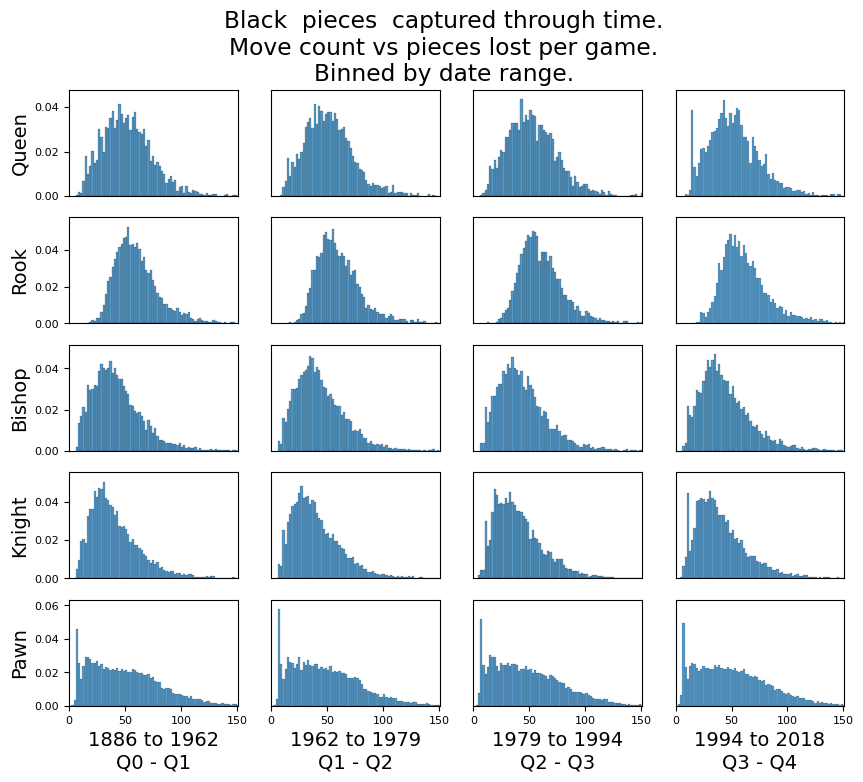
\includegraphics[width=\textwidth]{Images/_HIST_Queen_Rook_Bishop_Knight_Pawn_BLACK_DATE_TOURNEMENTS.png}
\end{center}

\subsection{DaenaliaEvandruile}
\label{sec:org4c1573b}
\begin{center}
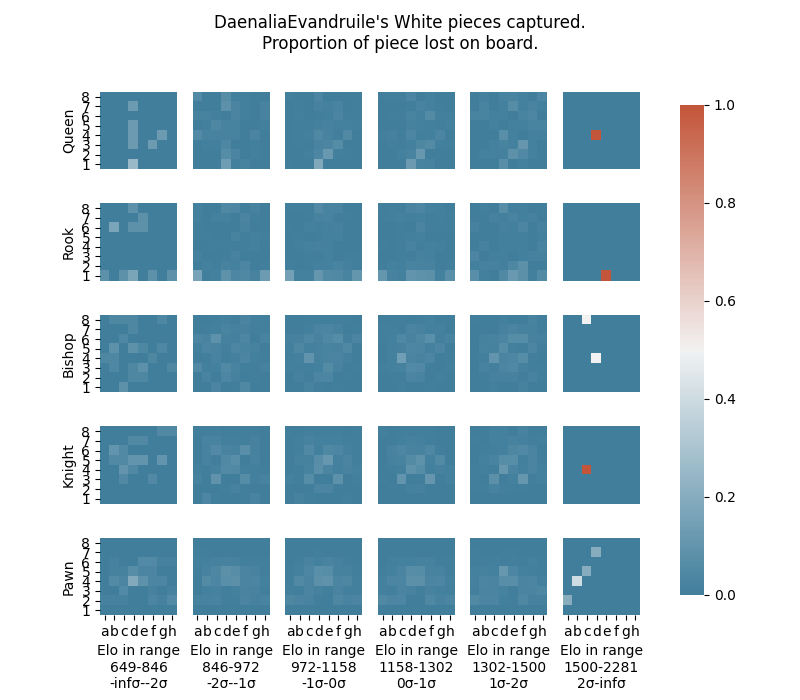
\includegraphics[width=\textwidth]{Images/DaenaliaEvandruile_HEATMAP_Queen_Rook_Bishop_Knight_Pawn_WHITE_ELO.png}
\end{center}

\begin{center}
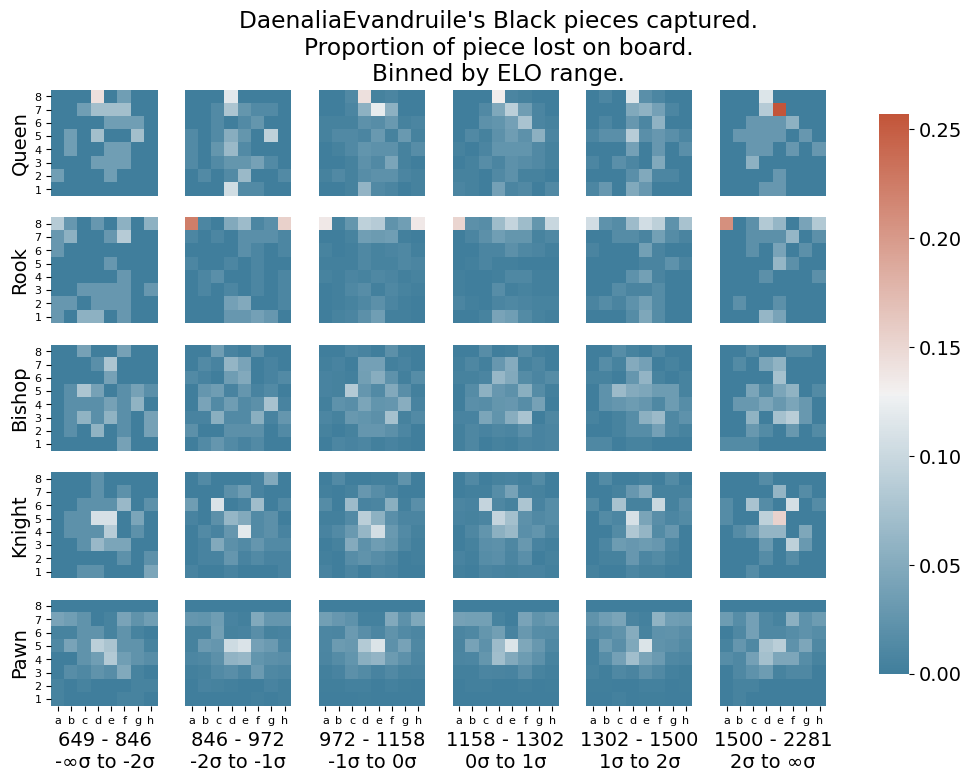
\includegraphics[width=\textwidth]{Images/DaenaliaEvandruile_HEATMAP_Queen_Rook_Bishop_Knight_Pawn_BLACK_ELO.png}
\end{center}


\begin{center}
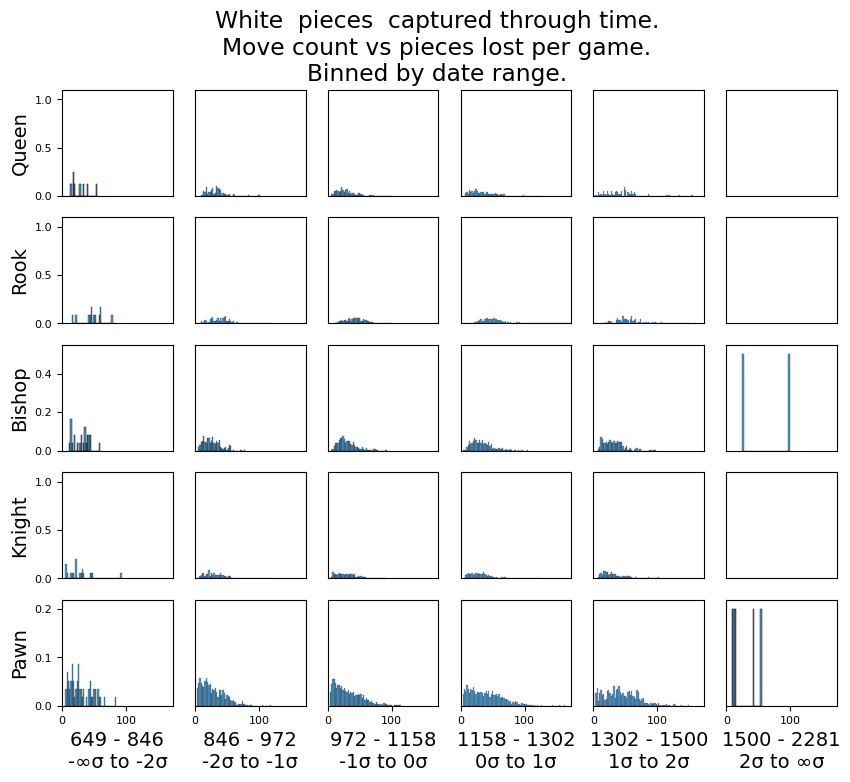
\includegraphics[width=\textwidth]{Images/DaenaliaEvandruile_HIST_Queen_Rook_Bishop_Knight_Pawn_WHITE_ELO.png}
\end{center}

\begin{center}
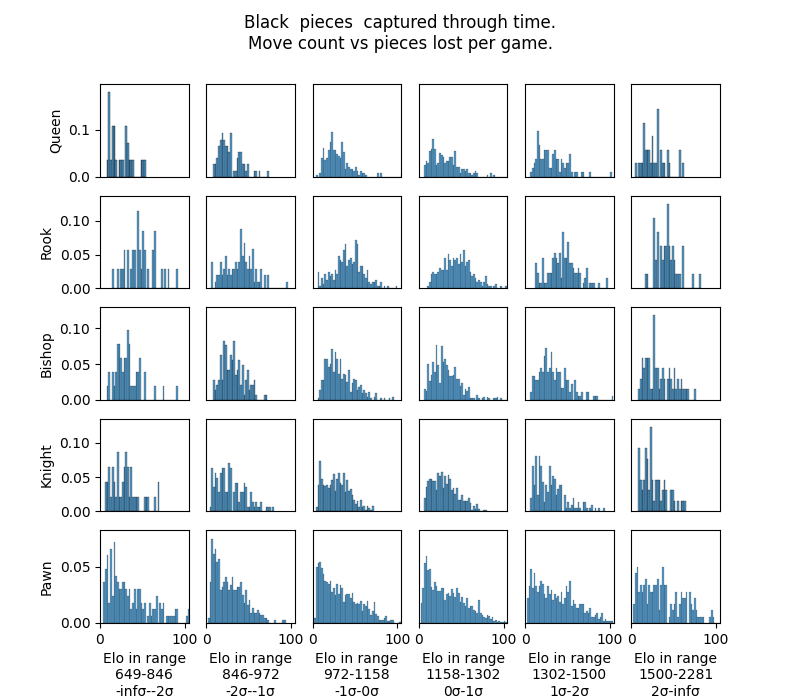
\includegraphics[width=\textwidth]{Images/DaenaliaEvandruile_HIST_Queen_Rook_Bishop_Knight_Pawn_BLACK_ELO.png}
\end{center}
\subsection{Individual piece plots}
\label{sec:org0718b0e}
\begin{center}
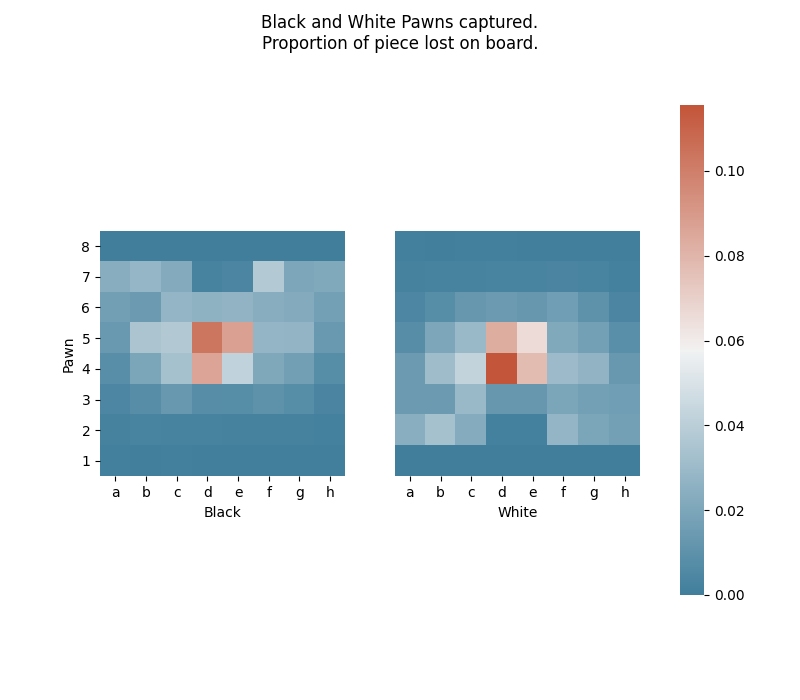
\includegraphics[width=0.4\textwidth]{Images/_HEATMAP_Pawn_FISC.png}
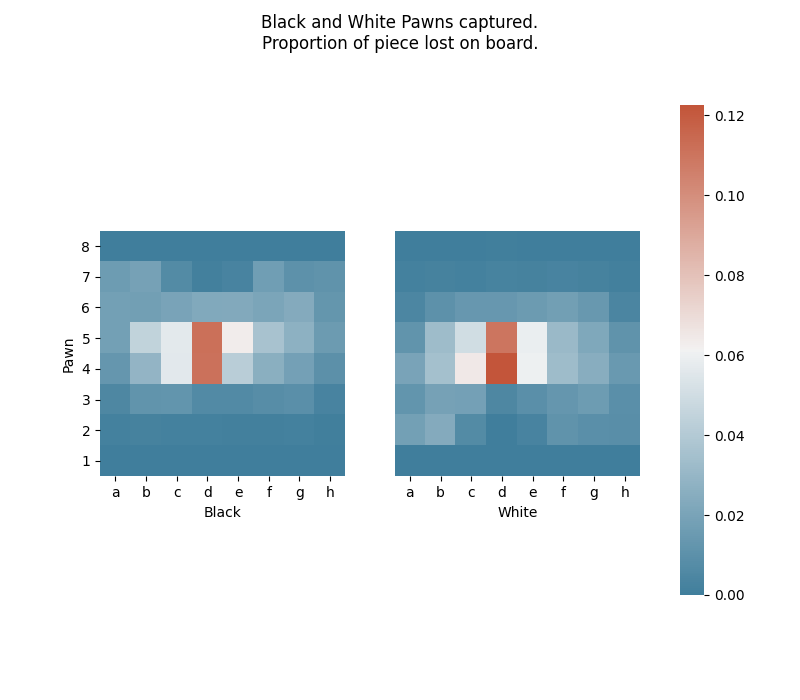
\includegraphics[width=0.4\textwidth]{Images/_HEATMAP_Pawn_TOURNEMENTS.png}
\end{center}
\begin{center}
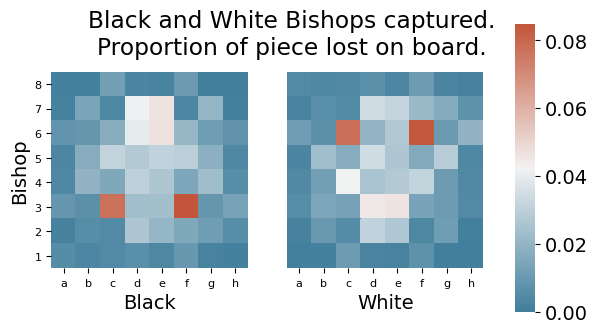
\includegraphics[width=0.4\textwidth]{Images/_HEATMAP_Bishop_FISC.png}
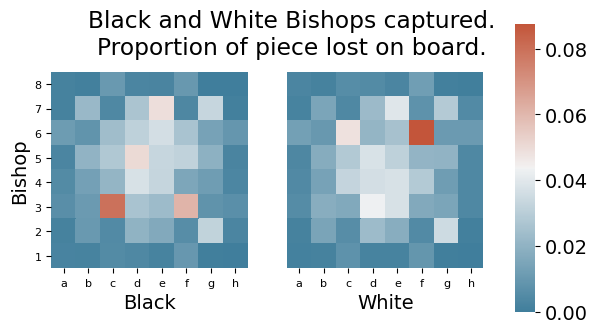
\includegraphics[width=0.4\textwidth]{Images/_HEATMAP_Bishop_TOURNEMENTS.png}
\end{center}
\begin{center}
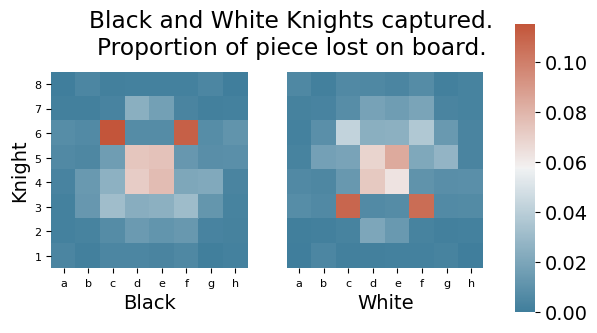
\includegraphics[width=0.4\textwidth]{Images/_HEATMAP_Knight_FISC.png}
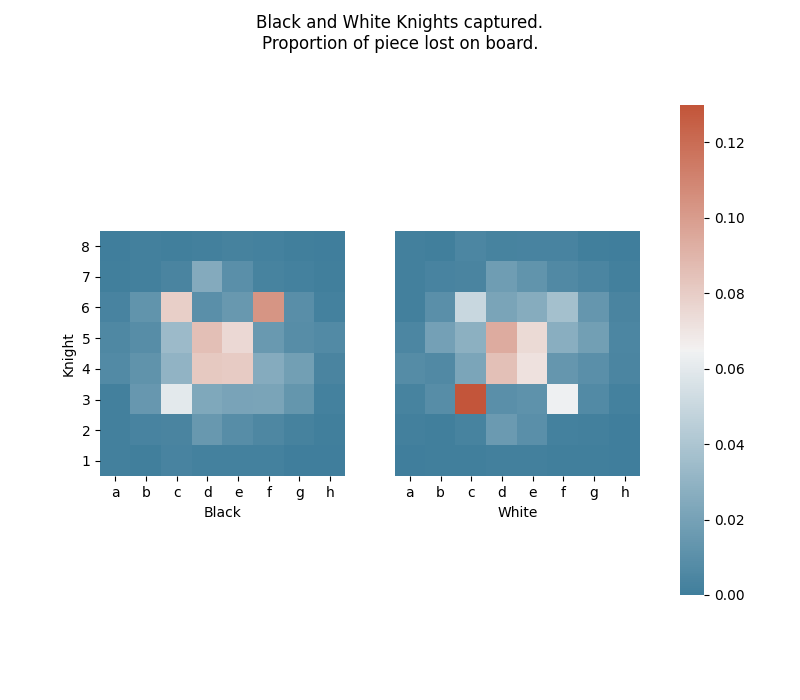
\includegraphics[width=0.4\textwidth]{Images/_HEATMAP_Knight_TOURNEMENTS.png}
\end{center}
\begin{center}
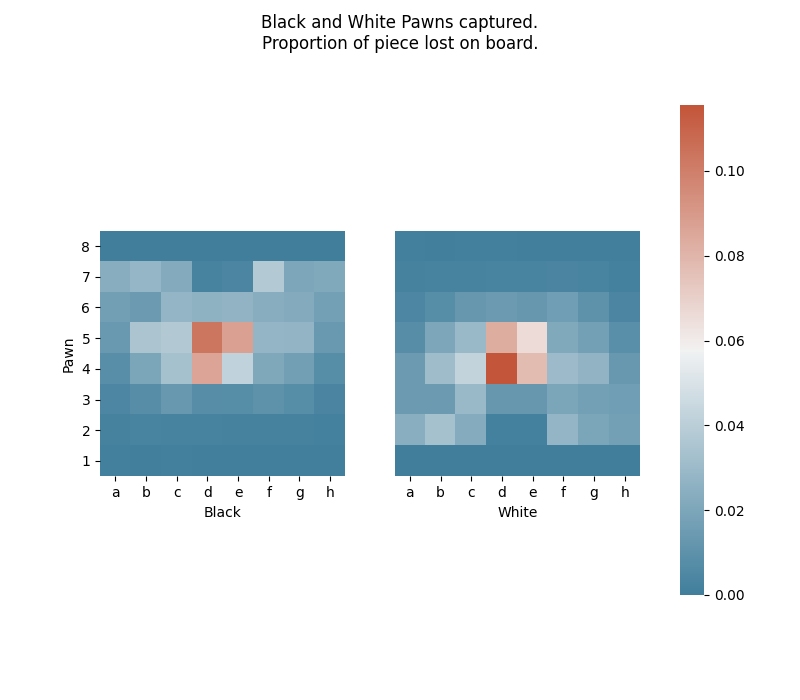
\includegraphics[width=0.4\textwidth]{Images/_HEATMAP_Pawn_FISC.png}
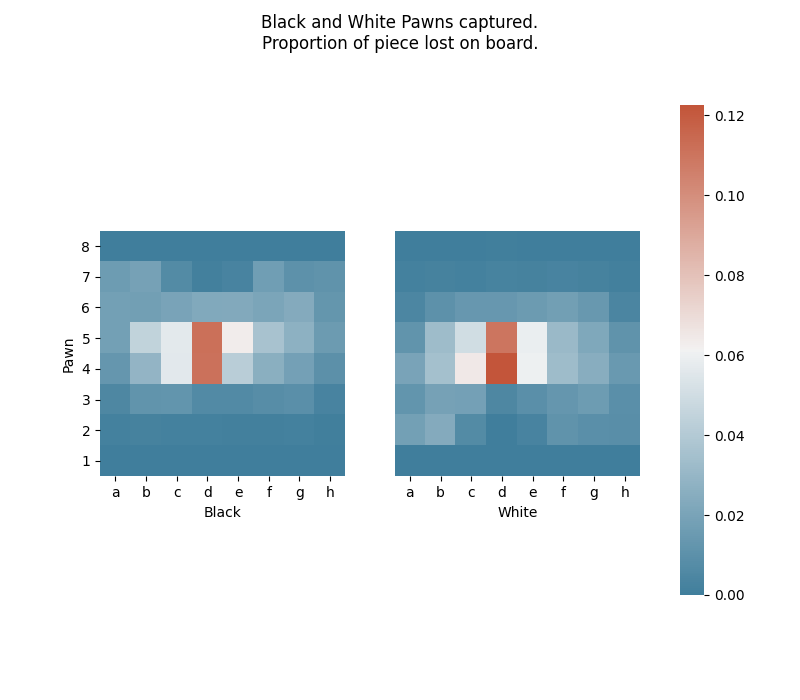
\includegraphics[width=0.4\textwidth]{Images/_HEATMAP_Pawn_TOURNEMENTS.png}
\end{center}
\begin{center}
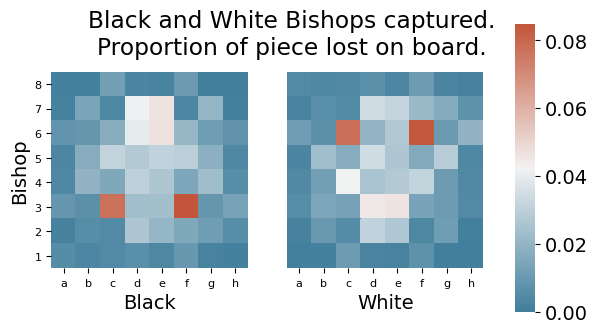
\includegraphics[width=0.4\textwidth]{Images/_HEATMAP_Bishop_FISC.png}
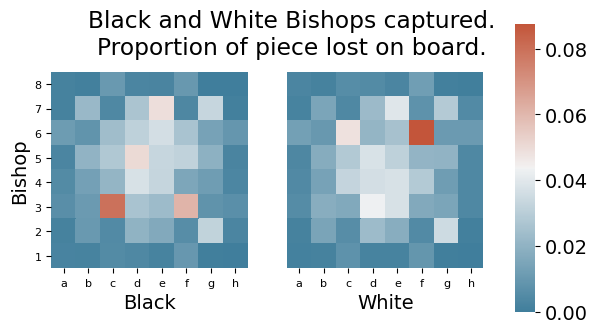
\includegraphics[width=0.4\textwidth]{Images/_HEATMAP_Bishop_TOURNEMENTS.png}
\end{center}
\begin{center}
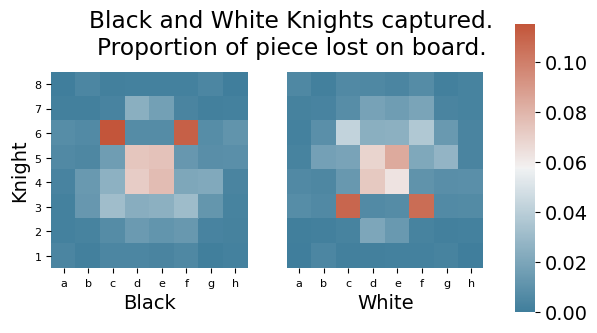
\includegraphics[width=0.4\textwidth]{Images/_HEATMAP_Knight_FISC.png}
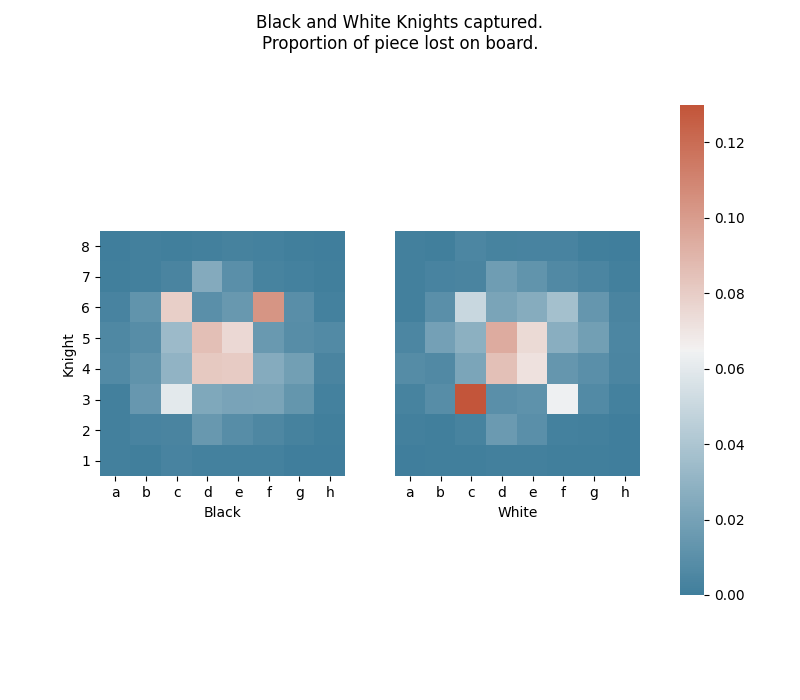
\includegraphics[width=0.4\textwidth]{Images/_HEATMAP_Knight_TOURNEMENTS.png}
\end{center}
\end{document}
